%        File: arfc-beamer.tex
%     Created: Sun May 5 10:00 PM 2013 C
%


%\documentclass[11pt,handout]{beamer}
\documentclass[9pt]{beamer}
\usetheme[white]{Illinois}
%\title[short title]{long title}
\title[ARFC Cyclus]{Cyclus Efforts in the Advanced Reactors and Fuel Cycles Group}
%\subtitle[short subtitle]{long subtitle}
\subtitle[Overview]{2018 Overview}
%\author[short name]{long name}
\author[Huff]{Kathryn Huff\\Advanced Reactors and Fuel Cycles Group}
%\date[short date]{long date}
\date[07.27.2018]{July 27, 2018}
%\institution[short name]{long name}
\institute[UIUC]{University of Illinois at Urbana-Champaign}

%\usepackage{bbding}
\usepackage{amsfonts}
\usepackage{amsmath}
\usepackage{xspace}
\usepackage{graphicx}
\usepackage{subfigure}
\usepackage{booktabs} % nice rules for tables
\usepackage{microtype} % if using PDF
\usepackage{bigints}
\usepackage{minted}

\newcommand{\units}[1] {\:\text{#1}}%
\newcommand{\SN}{S$_N$}%{S$_\text{N}$}%{$S_N$}%
\DeclareMathOperator{\erf}{erf}
%I need some complimentary error funcitons... 
\DeclareMathOperator{\erfc}{erfc}
%page numbers
\setbeamertemplate{footline}[page number]
\setbeamertemplate{caption}[numbered]
%Those icons in the references are terrible looking
\setbeamertemplate{bibliography item}[text]

%%%% Acronym support

\usepackage[acronym,toc]{glossaries}
\include{acros}

\makeglossaries

%try to get rid of header on title page\dots
\makeatletter
    \newenvironment{withoutheadline}{
        \setbeamertemplate{headline}[default]
        \def\beamer@entrycode{\vspace*{-\headheight}}
    }{}
\makeatother

\begin{document}
%%%%%%%%%%%%%%%%%%%%%%%%%%%%%%%%%%%%%%%%%%%%%%%%%%%%%%%%%%%%%
%% From uw-beamer Here's a handy bit of code to place at 
%% the beginning of your presentation (after \begin{document}):
\newcommand*{\alphabet}{ABCDEFGHIJKLMNOPQRSTUVWXYZabcdefghijklmnopqrstuvwxyz}
\newlength{\highlightheight}
\newlength{\highlightdepth}
\newlength{\highlightmargin}
\setlength{\highlightmargin}{2pt}
\settoheight{\highlightheight}{\alphabet}
\settodepth{\highlightdepth}{\alphabet}
\addtolength{\highlightheight}{\highlightmargin}
\addtolength{\highlightdepth}{\highlightmargin}
\addtolength{\highlightheight}{\highlightdepth}
\newcommand*{\Highlight}{\rlap{\textcolor{HighlightBackground}{\rule[-\highlightdepth]{\linewidth}{\highlightheight}}}}
%%%%%%%%%%%%%%%%%%%%%%%%%%%%%%%%%%%%%%%%%%%%%%%%%%%%%%%%%%%%%
%%--------------------------------%%
\begin{withoutheadline}
\frame{
  \titlepage
}
\end{withoutheadline}

%%--------------------------------%%
\AtBeginSection[]{
\begin{frame}
  \frametitle{Outline}
  \tableofcontents[currentsection]
\end{frame}
}

\section{Transition Scenarios}
\newcommand{\Cyclus}{\textsc{Cyclus}\xspace}%
\subsection{Predicting the Past: Spent Fuel Mass Validation}
\begin{frame}
  \frametitle{Predicting the Past: Spent Fuel Mass Validation}

\begin{block}{What is Predicting the Past? }
Use published data regarding 112 commercial nuclear reactors in the U.S. to create a \Cyclus simulation of the U.S. nuclear fuel cycle.
\end{block}


\begin{block}{Who}
Gwendolyn Chee, UIUC Graduate Student Researcher
\end{block}

\begin{block}{Where}
        \url{https://github.com/arfc/transition-scenarios} 
\end{block}
\end{frame}

\begin{frame}
\begin{block}{Current Work}
A comparison of spent fuel mass and isotopic compositions from the Predicting 
the Past \Cyclus output and spent nuclear fuel inventory from the U.S 
Department of Energy sponsored Unified Database\cite{peterson_unf-st&dards_2017} was conducted. This work has been submitted to ANS Winter 2018.
\end{block}

\begin{figure}[htbp!]
                \begin{center}
                        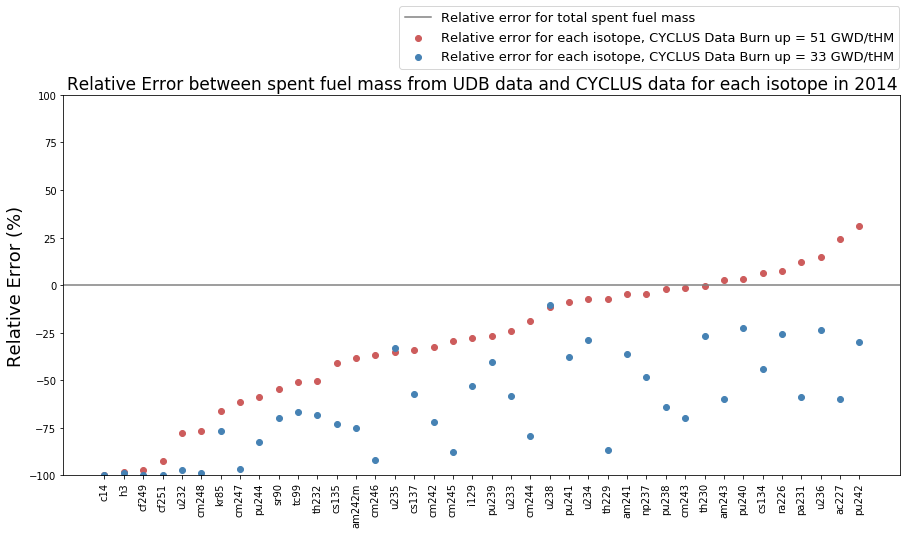
\includegraphics[height=0.7\textheight]{./images/relative_error_2014.png}
                        \caption{Relative error between \Cyclus prediction and 
                                CURIE data}
                \end{center}
        \end{figure}

\end{frame}


\subsection{Transition Benchmark}
\begin{frame}
  \frametitle{Transition Benchmark}
\begin{block}{What is the Transition Benchmark}
        Publish Cyclus contirbution to the ``Standardized Verification of Fuel 
        Cycle Modeling'' paper (Feng et al.)
\end{block}

\begin{block}{Who}
Jin Whan Bae, UIUC Graduate Student Researcher
\end{block}

\begin{block}{Where}
        \url{https://github.com/arfc/transition-scenarios} 

\end{block}

\end{frame}

\begin{frame}
  \frametitle{Transition Benchmark Results}

\begin{figure}[htbp!]
    \begin{center}
        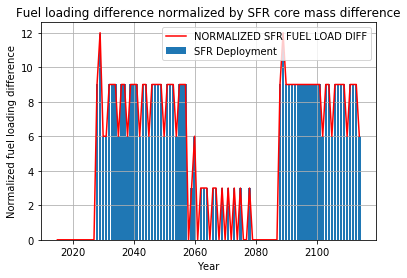
\includegraphics[scale=0.5]{./images/fuel_load_diff_norm.png}
    \end{center}
        \caption{Difference of annual fresh \gls{SFR} fuel loading rates (Cyclus - Benchmark) normalized by the core mass difference of an \gls{SFR} due to fractional batch size.}
    \label{fig:fuel_load_diff_norm}
\end{figure}

\end{frame}
\begin{frame}
  \frametitle{Transition Benchmark Results}
\begin{figure}[htbp!]
    \begin{center}
        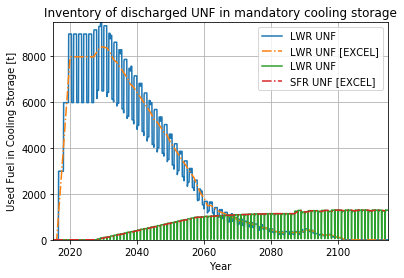
\includegraphics[scale=0.5]{./images/fuel_discharge_monthly.png}
    \end{center}
        \caption{Inventory of discharged UNF in mandatory cooling storage.}
    \label{fig:fuel_discharge_monthly}
\end{figure}

\end{frame}

\newcommand{\Cyclus}{\textsc{Cyclus}\xspace}%
\subsection{Predicting the Past}
\begin{frame}
  \frametitle{Predicting the Past: Spent Fuel Mass Validation}

\begin{block}{What is Predicting the Past? }
Predicting the Past uses published data of the 112 commercial nuclear reactors in the U.S. to create a \Cyclus simulation of the U.S. nuclear fuel cycle.
\end{block}

\begin{block}{Current Work}
Comparison between spent fuel mass and isotopic compositions from the predicting the past \Cyclus output and spent nuclear fuel inventory from the U.S Department of Energy sponsored Unified Database\cite{} was conducted. This work has been submitted to ANS Winter 2018.
\end{block}

\begin{block}{Who is working on this?}
Gwendolyn Chee, UIUC Graduate Student Researcher
\end{block}

\begin{block}{Where is Predicting the Past?}
Predicting the Past and the validation results can be found in: \href{https://github.com/arfc/transition-scenarios/tree/master/input/predicting-the-past}{arfc/transition-scenarios} 
\end{block}

\end{frame}
\section{Tutorial}
\input{tutorial}
\section{Cyder}
\subsection{Cyder2.0: Goals and Current Work}
\begin{frame}
  \frametitle{Cyder2.0}

\begin{block}{Goals for Cyder2.0}
\begin{enumerate}
	\item Create a Waste Conditioning Facility archetype and a Simple Heat-Limited Repository archetype that can be optimized to load waste packages into the repository based on a thermal constraints. 
	\item Add both archetypes into the Predicting the Past \Cyclus simulation to simulate loading U.S. nuclear waste packages into a final waste repository. 
\end{enumerate}
\end{block}

\begin{block}{Current Work}
	Creating the Conditioning Facility archetype
\end{block}

\begin{block}{How the Conditioning Facility archetype works}
The user can specify the commodity and material resource object that the archetype accepts and produces. Based on that, the archetype conditions the input and puts it into the form of the user-specified output.
\end{block}

\end{frame}

\subsection{Cyder2.0:Expectations}

\begin{frame}
\frametitle{Cyder2.0}

\begin{block}{When will it be ready?}
	Waste Conditioning Archetype: August 2018 \\
	Simple Heat-Limited Repository Archetype: October 2018 
\end{block}

\begin{block}{Who is working on this?}
	Gwendolyn Chee, UIUC Graduate Student Researcher
\end{block}

\begin{block}{Where is Cyder?}
	Cyder can be found in: \href{https://github.com/arfc/cyder}{arfc/cyder} 
\end{block}

\end{frame}
\section{Demand Driven Cycamore Archetypes}
\newcommand{\Cyclus}{\textsc{Cyclus}\xspace}%
\subsection{What is it?}
\begin{frame}
  \frametitle{}
  % a comment

\begin{block}{Goals for the Demand Driven Cycamore Archetype}
\begin{enumerate}
	\item Give \Cyclus the capability to deploy supporting fuel cycle facilities to meet front-end and back-end demands of the fuel cycle. 
	\item Develop three types of prediction algorithms to achieve this capability: Non-optimizing, Deterministic Optimizing, Stochastic Optimizing. Each will improve on the previous algorithm to make the predictions more accurate. 
\end{enumerate}
\end{block}

\begin{block}{How it works}
User-specified inputs: 
\begin{enumerate}
	\item A commodity that the user wants to demand. 
	\item Growth rate of that specific commodity 
	\item The facilities in the simulation and their corresponding parameters
\end{enumerate}
Using the user-specified inputs, the archetype will deploy facilities and supporting facilities to meet the demand for the specified commodity and the supporting commodities required to produce it. 
\end{block}


\end{frame}

\subsection{Current work}
\begin{frame}
\frametitle{}
% a comment

\begin{block}{People involved in this project}
	\textbf{University of South Carolina}\\
	PI: Dr. Anthony Scopatz \\
	Postdoc Researcher: Dr. Robert Flanagan \\
	\textbf{University of Illinois at Urbana Champaign} \\
	Co-PI: Dr. Kathryn Huff \\
	Graduate Student Researchers: Gwendolyn Chee and Jin Whan Bae (Teddy)
\end{block}

\begin{block}{Current work being done by UIUC}
	\begin{enumerate}
		\item Numerical experiments to test the non-optimizing and deterministic optimizing prediction algorithms. 
		\item A Report for each type of prediction algorithm. The report for the non-optimizing case can be found \cite{bae_numerical_2018}
	\end{enumerate}
\end{block}

\begin{block}{When will it be ready? }
	Non-Optimizing Algorithm: August 2018	\\
	Deterministic-Optimizing Algorithm: October 2018	
\end{block}


\end{frame}

\section{PyRe}
%        File: arfc-beamer.tex
%     Created: Sun May 5 10:00 PM 2013 C
%


%\documentclass[11pt,handout]{beamer}
\documentclass[9pt]{beamer}
\usetheme[white]{Illinois}
%\title[short title]{long title}
\title[Short Title]{A Very Very Long Title for a Presentation about Cats}
%\subtitle[short subtitle]{long subtitle}
\subtitle[Short SubTitle]{Mostly Kittens}
%\author[short name]{long name}
\author[Your Name]{Your Name\\Advanced Reactors and Fuel Cycles Group}
%\date[short date]{long date}
\date[04.01.2100]{April 1, 2100}
%\institution[short name]{long name}
\institute[UIUC]{University of Illinois at Urbana-Champaign}

%\usepackage{bbding}
\usepackage{amsfonts}
\usepackage{amsmath}
\usepackage{xspace}
\usepackage{graphicx}
\usepackage{subfigure}
\usepackage{booktabs} % nice rules for tables
\usepackage{microtype} % if using PDF
\usepackage{bigints}
\usepackage{tabularx}
%\usepackage{minted}

\newcommand{\units}[1] {\:\text{#1}}%
\newcommand{\SN}{S$_N$}%{S$_\text{N}$}%{$S_N$}%
\DeclareMathOperator{\erf}{erf}
%I need some complimentary error funcitons... 
\DeclareMathOperator{\erfc}{erfc}
%page numbers
\setbeamertemplate{footline}[page number]
\setbeamertemplate{caption}[numbered]
%Those icons in the references are terrible looking
\setbeamertemplate{bibliography item}[text]

%%%% Acronym support

\usepackage[acronym,toc]{glossaries}
\include{acros}

\makeglossaries

%try to get rid of header on title page\dots
\makeatletter
    \newenvironment{withoutheadline}{
        \setbeamertemplate{headline}[default]
        \def\beamer@entrycode{\vspace*{-\headheight}}
    }{}
\makeatother
\begin{document}
	%%%%%%%%%%%%%%%%%%%%%%%%%%%%%%%%%%%%%%%%%%%%%%%%%%%%%%%%%%%%%
	%% From uw-beamer Here's a handy bit of code to place at 
	%% the beginning of your presentation (after \begin{document}):
	\newcommand*{\alphabet}{ABCDEFGHIJKLMNOPQRSTUVWXYZabcdefghijklmnopqrstuvwxyz}
	\newlength{\highlightheight}
	\newlength{\highlightdepth}
	\newlength{\highlightmargin}
	\setlength{\highlightmargin}{2pt}
	\settoheight{\highlightheight}{\alphabet}
	\settodepth{\highlightdepth}{\alphabet}
	\addtolength{\highlightheight}{\highlightmargin}
	\addtolength{\highlightdepth}{\highlightmargin}
	\addtolength{\highlightheight}{\highlightdepth}
	\newcommand*{\Highlight}{\rlap{\textcolor{HighlightBackground}{\rule[-\highlightdepth]{\linewidth}{\highlightheight}}}}
	%%%%%%%%%%%%%%%%%%%%%%%%%%%%%%%%%%%%%%%%%%%%%%%%%%%%%%%%%%%%%
	%%--------------------------------%%
	\begin{frame}
	\frametitle{PyRe: Cyclus (Py)ro (Re)processing Module}
	\begin{columns}
		\begin{column}{.45\textwidth}
			\textbf{Current Work:} \\
			Create a class for each sub-process, and build the archetype. \\
			\vspace{1mm}
			\textbf{How does PyRe work?} \\
			PyRe does the following with an input stream and facility configuration parameters: 
			\begin{itemize}
				\item Fuel passed into voloxidation subprocess.
				\item A table of separation efficiencies is generated from input parameters.
				\item Input stream is multiplied by efficiency table to separate waste.
				\item Repeated for each process - results in product and waste composition streams.
			\end{itemize}
		\end{column}
		\begin{column}{.55\textwidth}
			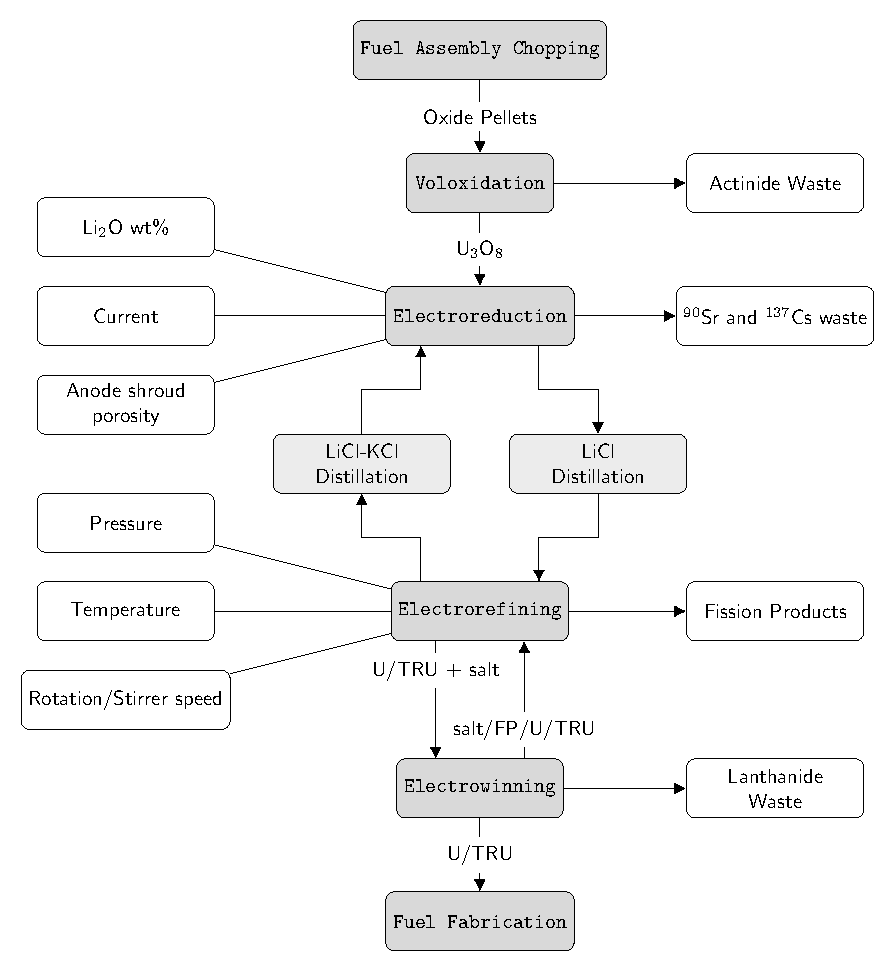
\includegraphics[width=\linewidth]{flowchart}
		\end{column}
	\end{columns}
	\end{frame}
	\begin{frame}
	\frametitle{PyRe: Cyclus (Py)ro (Re)processing Module}
	\textbf{Timeline:} \\
	The archetype will be functional with preliminary efficiencies early \textbf{August 2018}. \\
	A more detailed PyRe will be completed for ANTPC in \textbf{September 2018}. \\
	\vspace{1mm}
	\textbf{Archetype Uses:} \\
	PyRe will answer the following questions
	\begin{itemize}
			\item What is the affect of introducing pyroprocessing plants in the fuel cycle?
			\item How various facility designs affect throughput, efficiency and fabrication time?
			\item What are the best points to monitor a pyroprocessing plant for diversion?
	\end{itemize}
	\vspace{1mm}
	\textbf{Where is PyRe?} \\
	PyRe can be found in the "pyre" branch of recycle: \href{https://github.com/arfc/recycle}{arfc/recycle.} \\
	\vspace{1mm}
	\textbf{Who is working on this?}\\
	Greg Westphal, UIUC Graduate Researcher \\
	
	\end{frame}
\end{document}
\section{Conclusion}
\input{conclusion}
\input{acks}
%%--------------------------------%%
%%--------------------------------%%
\begin{frame}[allowframebreaks]
  \frametitle{References}
  \bibliographystyle{plain}
  {\footnotesize \bibliography{2018-07-27-cyclus-call.bib} }

\end{frame}

%%--------------------------------%%


\end{document}



